\section{Introduction}

\subsection{Theory}

Resistance can be measured using two methods: direct or indirect. 

\subsubsection*{Direct}

To take a direct measurement, the measured component must be connected to the ohmmeter as shown in Fig.~\ref{fig:direct_schematic}. The component cannot be connected to a circuit, and must be passive and linear. A linear component isn't influenced by other parameters and will not change its value over time.

\begin{figure}[H]
	\centering
	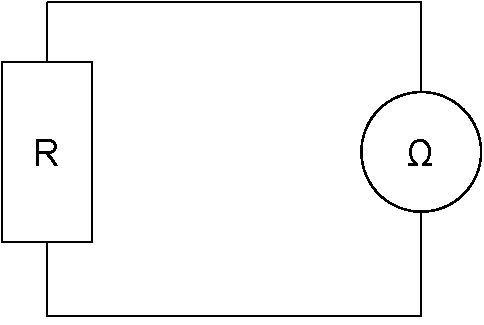
\includegraphics[width=6cm]{schematics/direct.pdf}
	\caption{Direct resistance measurement schematic}
	\label{fig:direct_schematic}
\end{figure}

\subsubsection*{Indirect}

Resistance is measured indirectly using the ammeter-voltmeter method. Figures~\ref{fig:CVM},~\ref{fig:CCM} show different ways of implementing said method. In both instances, the resistance is calculated using the Ohm's law: $R=\frac{U}{I}$.  

\begin{figure}[H]
	\centering
	\begin{minipage}{.4\textwidth}
		\centering
		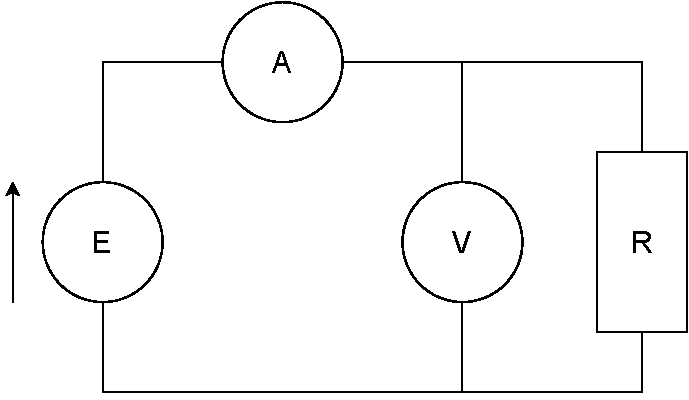
\includegraphics[width=1\linewidth]{schematics/CVM.pdf}
	\end{minipage}\qquad
	\begin{minipage}{.4\textwidth}
		\centering
		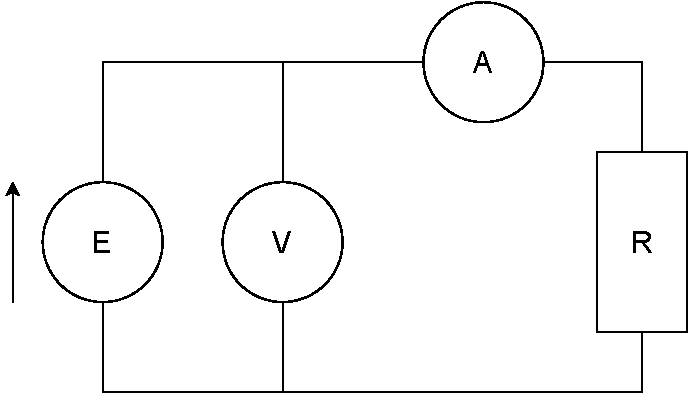
\includegraphics[width=1\linewidth]{schematics/CCM.pdf}
	\end{minipage}
	
	\bigskip
	
	\begin{minipage}[t]{.4\textwidth}
		\centering
		
		\caption{CVM (circuit with correct voltage measurement)}
		\label{fig:CVM}
	\end{minipage}\qquad
	\begin{minipage}[t]{.4\textwidth}
		\centering
		\caption{CCM (circuit with correct current measurement)}
		\label{fig:CCM}
	\end{minipage}
\end{figure}

The method error is calculated using the following formulas:
\begin{itemize}
	\item CVM: $\Delta_m R = \frac{-R_m^2}{R_V - R_m}$, $\delta_m R = \frac{-R_m}{R_V}$;
	\item CCM: $\Delta_m R = R_A$, $\delta_m R = \frac{R_A}{R_m - R_A}$;
\end{itemize}

The CVM circuit should be used for small resistances and the CCM circuit should be used for big resistances. The following equation describes the threshold resistance for which the choice of the circuit doesn't matter: $R_{thr} = \sqrt{R_V\cdot R_A}$.


\subsection{Equipment}

The following devices were used during the laboratory:

\begin{itemize}
	\item power supply: DF1730SB3A;
	\item digital meter: Agilent 34401A;
	\item decade resistor: DR4b-16;
	\item digital meter: UT803;
	\item linear resistor;
	\item diode resistor.
	\item analog voltmeter: LM-3;
	\item analog ammeter: LM-3.
\end{itemize}